\def\PZ{\ensuremath{\mathrm{Z}}\xspace}
\def\PV{\ensuremath{\mathrm{V}}\xspace}
\def\ZZ{\ensuremath{\PZ\PZ}\xspace}
\def\WW{\ensuremath{\PW\PW}\xspace}
\def\WZ{\ensuremath{\PW\PZ}\xspace}
\def\QT{\ensuremath{q_{\mathrm{T}}}\xspace}
\def\PT{\ensuremath{p_{\mathrm{T}}}\xspace}
\def\VECPT{\ensuremath{\vec{p}_{\mathrm{T}}}\xspace}
\def\VECQT{\ensuremath{\vec{q}_{\mathrm{T}}}\xspace}
\def\ET{\ensuremath{E_{\mathrm{T}}}\xspace}
\def\MET{\ensuremath{{E\!\!\!/}_{\mathrm{T}}}}
\def\PFMET{\ensuremath{\MET}}
\def\PUMET{\ensuremath{{\MET}^{\mathrm{PU}}}}
\def\PUMETMIN{\ensuremath{{\MET}^{\mathrm{PU,min}}}}
\def\CORRMET{\ensuremath{{\MET}^{\mathrm{corr}}}}

\def\SIGBRZZee{\ensuremath{ [\,\sigma\times {\cal{B}}\,](\ \, \pp\to \ZZ \to \Pe\Pe\nu\nu\ ) }\xspace } 
\def\SIGBRZZmm{\ensuremath{ [\,\sigma\times {\cal{B}}\,](\, \pp\to \ZZ \to \Pgm\Pgm\nu\nu\ ) }\xspace } 
\def\SIGBRZZll{\ensuremath{ [\,\sigma\times {\cal{B}}\,](\ \, \pp\to \ZZ \to \ell\ell\nu\nu\ ) }\xspace } 
\def\SIGZZ{\ensuremath{ \sigma( \pp\to\ZZ )  }\xspace}

\def\NbkgEleWjets{ \ensuremath{ 3.4 \pm 1.1 \pm 1.5 }\xspace } 
\def\NbkgEleWGam{ \ensuremath{ 1.5 \pm 0.4  }\xspace } 
\def\NbkgEleTop{   \ensuremath{ 0.7 \pm 0.4 }\xspace } 
\def\NbkgEleNonPeaking{ \ensuremath{ 5.6 \pm 2.1 }\xspace } 
\def\NbkgElePeakingZJ{ \ensuremath{ 3.6 \pm 0.9 }\xspace } 
\def\NbkgElePeakingZG{ \ensuremath{ 0.3 \pm 0.2 }\xspace } 

\def\NElePeaking{ \ensuremath{ 11.2 \pm 5.2\,{\mathrm{(stat)}} \pm 1.6\,{\mathrm{(bkg)}} }\xspace }
\def\NElePeakingWithWZ{ \ensuremath{ 14.4 \pm 5.2\,_{\mathrm{(stat)}} \pm 1.1\,_{\mathrm{(bkg)}} }\xspace }
\def\NEleNonPeaking{ \ensuremath{ 14.1 \pm 5.2\,_{\mathrm{(stat)}} \pm 1.6\,_{\mathrm{(bkg)}} }\xspace }

\def\NbkgMuoWjets{ \ensuremath{ 0.0\,^{+0.9}_{-0.0} }\xspace }
\def\NbkgMuoTop{   \ensuremath{ 1.0 \pm 0.5 }\xspace } 
\def\NbkgMuoNonPeaking{ \ensuremath{ 1.0\,^{ \pm 1.4 }_{-0.5} }\xspace } 
\def\NbkgMuoPeakingZJ{ \ensuremath{ 1.6 \pm 0.4 }\xspace } 
\def\NbkgMuoPeakingZG{ \ensuremath{ 0.1 \pm 0.1 }\xspace } 

\def\NMuoPeaking{ \ensuremath{ 10.4 \pm 4.8\,{\mathrm{(stat)}}\pm 1.1\,{\mathrm{(bkg)}}  }\xspace }
\def\NMuoPeakingWithWZ{ \ensuremath{ 13.6 \pm 4.8\,_{\mathrm{(stat)}}\pm 0.5\,_{\mathrm{(bkg)}}  }\xspace }
\def\NMuoNonPeaking{ \ensuremath{ 17.9 \pm 5.1\,_{\mathrm{(stat)}} \pm 1.0\,_{\mathrm{(bkg)}} }\xspace }

\def\NbkgZWInZZee{ \ensuremath{ 3.2 \pm 0.5 }\xspace }
\def\NbkgZWInZZmm{ \ensuremath{ 3.2 \pm 0.6 }\xspace }

\def\RhoEleZZ{ \ensuremath{ 0.714 \pm 0.007 }\xspace }
\def\RhoMuoZZ{ \ensuremath{ 0.779 \pm 0.007 }\xspace }
\def\RhoEleWZ{ \ensuremath{ 0.725 \pm 0.010 }\xspace }
\def\RhoMuoWZ{ \ensuremath{ 0.790 \pm 0.010 }\xspace }

\def\ZZElecXsect{\ensuremath{ 180 \pm 54\,_{\mathrm{(stat)}}\, \pm 34\,_{\mathrm{(syst)}}\, \pm 11\,_{\mathrm{(lumi)}} \ \mathrm{fb} }\xspace }
\def\ZZMuonXsect{\ensuremath{ 122 \pm 38\,_{\mathrm{(stat)}}\, \pm 20\,_{\mathrm{(syst)}}\, \pm \ \, 7\,_{\mathrm{(lumi)}} \ \mathrm{fb} }\xspace }
\def\ZZCombXsect{\ensuremath{ 151 \pm 47\,_{\mathrm{(stat)}}\, \pm 27\,_{\mathrm{(syst)}}\, \pm \ \, 9\,_{\mathrm{(lumi)}} \ \mathrm{fb} }\xspace }

\def\ZZXsect{\ensuremath{ 11.2 \pm 3.5\,_{\mathrm{(stat)}}\, \pm 2.0\,_{\mathrm{(syst)}}\, \pm 0.7\,_{\mathrm{(lumi)}} \ \mathrm{pb} }\xspace }

% aTGCs
\def\FqLimTwoSig{\ensuremath{\displaystyle -0.080 < f_{4}^{Z}  < 0.080 }\xspace }
\def\FcLimTwoSig{\ensuremath{\displaystyle -0.077 < f_{5}^{Z}  < 0.077 }\xspace }
\def\FqLimOneSig{\ensuremath{\displaystyle -0.051 < f_{4}^{Z}  < 0.051 }\xspace }
\def\FcLimOneSig{\ensuremath{\displaystyle -0.051 < f_{5}^{Z}  < 0.051 }\xspace }


\section{$\PZ\PZ$ in the $\ell\ell\nu\nu$ channel}

This section describes the study of the $\PZ\PZ$ diboson production in the channel where one of the $\PZ$-boson decays to charged leptons ($\PZ\to\ell\ell$, with $\ell=\Pe,\,\Pgm$) while the other decays to a pair of neutrinos ($\PZ\to\nu\nu$).  The signal is characterized by the presence of one reconstructed $\PZ\to\ell\ell\,$ boson, whose transverse momentum is balanced by the missing transverse momentum associated to the escaping neutrinos. The branching fraction for the $\PZ\PZ\to\ell\ell\nu\nu$ channel is more then six times larger than for the $\ZZ\to4\ell$ channel; furthermore, the neutrinos are not affected by detector acceptance. The backgrounds, however, are also much larger. The main backgrounds are Drell-Yan, due to the finite $\met$ resolution; $\PZ+{\mathrm {jets}}$, where the jet is lost or mis-measured; $\PZ+\gamma$, where the photon is lost; $t\bar{t}$ and single-top, where the leptons and $\met$ come from $\PW$ decays; $\WW$, for the same reasons; and $\WZ$, when the lepton from the $\PW$ decay is lost.  There are other smaller backgrounds involving $\PZ\to\tau\tau$ decays or fake electrons.
%, but they are found to be negligible, although we use control samples to check this assumption.

The present analysis is based on $\mathcal{L} = 1070\pm64~\mathrm{pb}^{-1}$ of data collected by the CMS experiment in 2011.

\subsection{Event Selection and Signal Extraction}

We consider samples triggered by the double-electron and double-muon high-level trigger lines and we select events with two lepton candidates of same flavor and opposite charge in the $[\,60$ - $120\,]~\GeV$ invariant mass window. We request leptons to have transverse momenta larger than $20~\GeV$. In the electron decay channel,  both electrons are  identified with tight identification and isolation criteria in order to reduce the contribution of QCD multi-jet and $\PW+{\mathrm {jets}}$ background events.  In the muon channel, only one of the muons is identified with tight criteria.  

The two leptons are required to originate from a common vertex, defined as the {\it hard-scatter} vertex. We use the number of additional reconstructed vertices as a measure of the pile-up activity in the event. This number is five in average, but can be as large as twenty, for the considered data set. 

Each charged particle candidate is associated to one of the vertices, on the basis of the closest distance of its trajectory to the vertex position in 3D-space.  Isolated photon candidates with $\ET^{\gamma}>30~\GeV$ are associated to the hard-scatter vertex; all other photons are attributed to the pile-up.  

Hadronic jets are clustered  from the list of charged and neutral candidates prepared by the particle-flow (PF) algorithm, using the anti-kT algorithm with a cone size of 0.5. Only calibrated jets with  $|\eta^{\mathrm{jet}}|<5$ and $\ET^{\mathrm{jet}}>10~\GeV$ are considered.  A jet with $\ET^{\mathrm{jet}}>30~\GeV$, or matching the recoil of the di-lepton candidate, is associated to the hard-scatter vertex. A jet within tracker acceptance ($|\eta^{\mathrm{jet}}|<2.4$) is associated to the reconstructed vertex that minimizes $\Sigma \PT$, where the scalar sum runs over transverse momenta of charged track constituents associated to that vertex. All other jets and unclustered charged or neutral PF candidates are attributed to the pile-up.

\begin{figure}[bt]
\begin{minipage}[t]{0.48\linewidth}
\centering
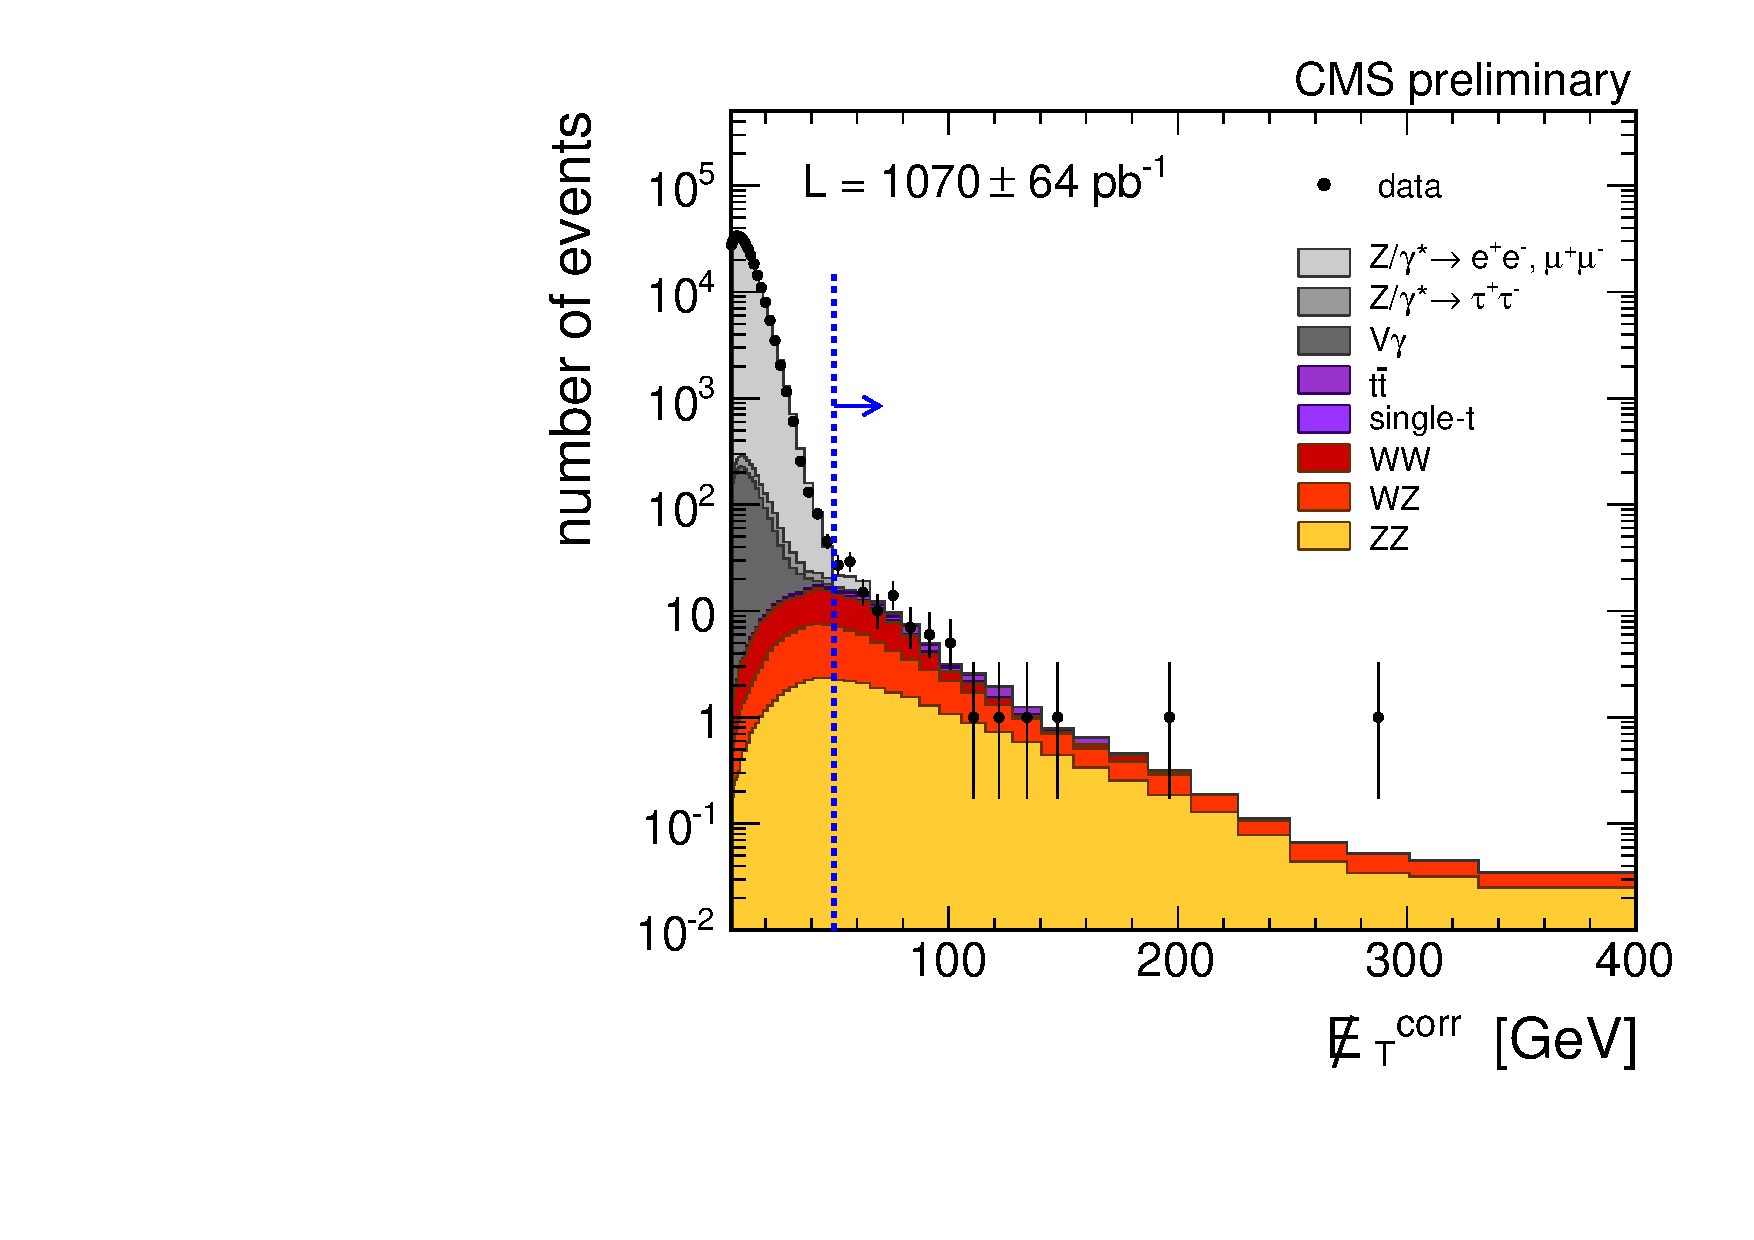
\includegraphics[width=1\linewidth]{figures/ZZ_2l2n/corrMET_jet.pdf}
%\hspace{.05in}
\caption{Distribution of the corrected $\met$ variable for di-lepton events after the jet veto. The cut at $50~\GeV$ is indicated by a dashed blue line. \label{fig:ZZ_2l2n_corrMET_jet}}
%\end{center}
\end{minipage}
\hspace{0.5cm}
\begin{minipage}[t]{0.48\linewidth}
\centering
%\begin{center}
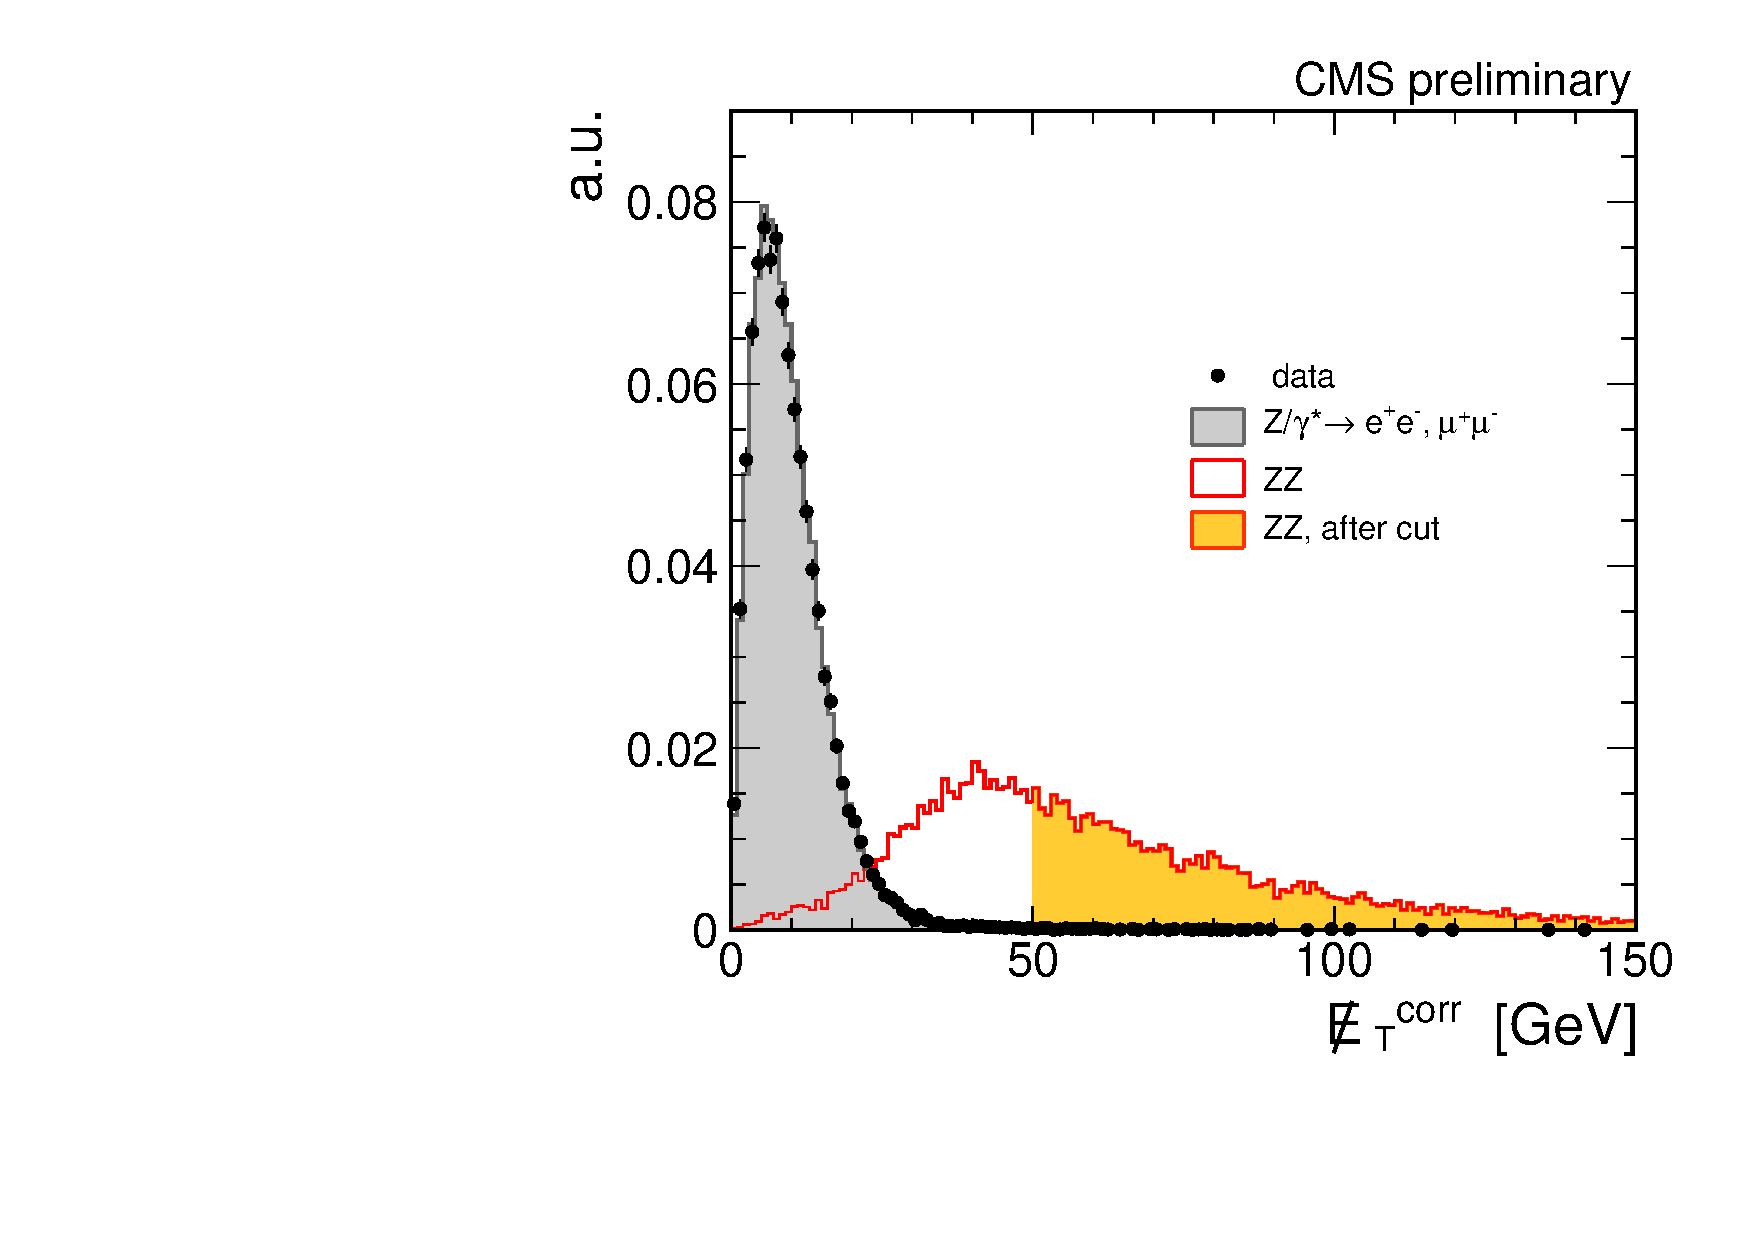
\includegraphics[width=1\linewidth]{figures/ZZ_2l2n/corrMET_q30_jet.pdf}
\caption{Distribution of the corrected $\met$ variable for di-lepton events after the jet veto and the $\QT>30~\GeV$ cut for the data (dots), the Drell Yan simulation (in gray) and the \ZZ\ signal (in red). The distributions are normalized to unity.  \label{fig:ZZ_2l2n_corrMET_q30_jet}}
\end{minipage}
\end{figure}

We consider several missing transverse energy variables. The standard \PFMET\ is constructed as the modulus of $-\Sigma \VECPT$, where the vector sum runs over transverse momenta of calibrated jets and unclustered charged or neutral PF candidates.  In the second variable, called \PUMET, the contribution to the vector sum of objects associated to the pile-up is scaled down by the number of additional vertices. Although the \PUMET\ variable is less sensitive to the conditions of pile-up, it can take erroneously-large values due to possible mis-associations of jets or unclustered PF candidates to the wrong vertices.  To avoid the development of tails in the $\met$ distribution, we form the minimum of the \PFMET\ and \PUMET\ variables. The resulting \PUMETMIN\ variable shows much improved discrimination against the Drell-Yan background compared to the first two variables.  We use a parameterization of the residual dependence of the \PUMETMIN\ variable as a function of the number of additional vertices to obtain a rescaled variable \CORRMET, defined so that the distribution of \PUMETMIN\ for Drell-Yan events in the data without pile-up be unchanged. By construction, a cut on the \CORRMET\ variable presents the same rejection power against Drell-Yan events irrespective of the pile-up conditions, in the electron and muon channels, in the data and the Monte-Carlo simulation.

\begin{figure}[bt]
\begin{minipage}[t]{0.48\linewidth}
\centering
%\begin{center}
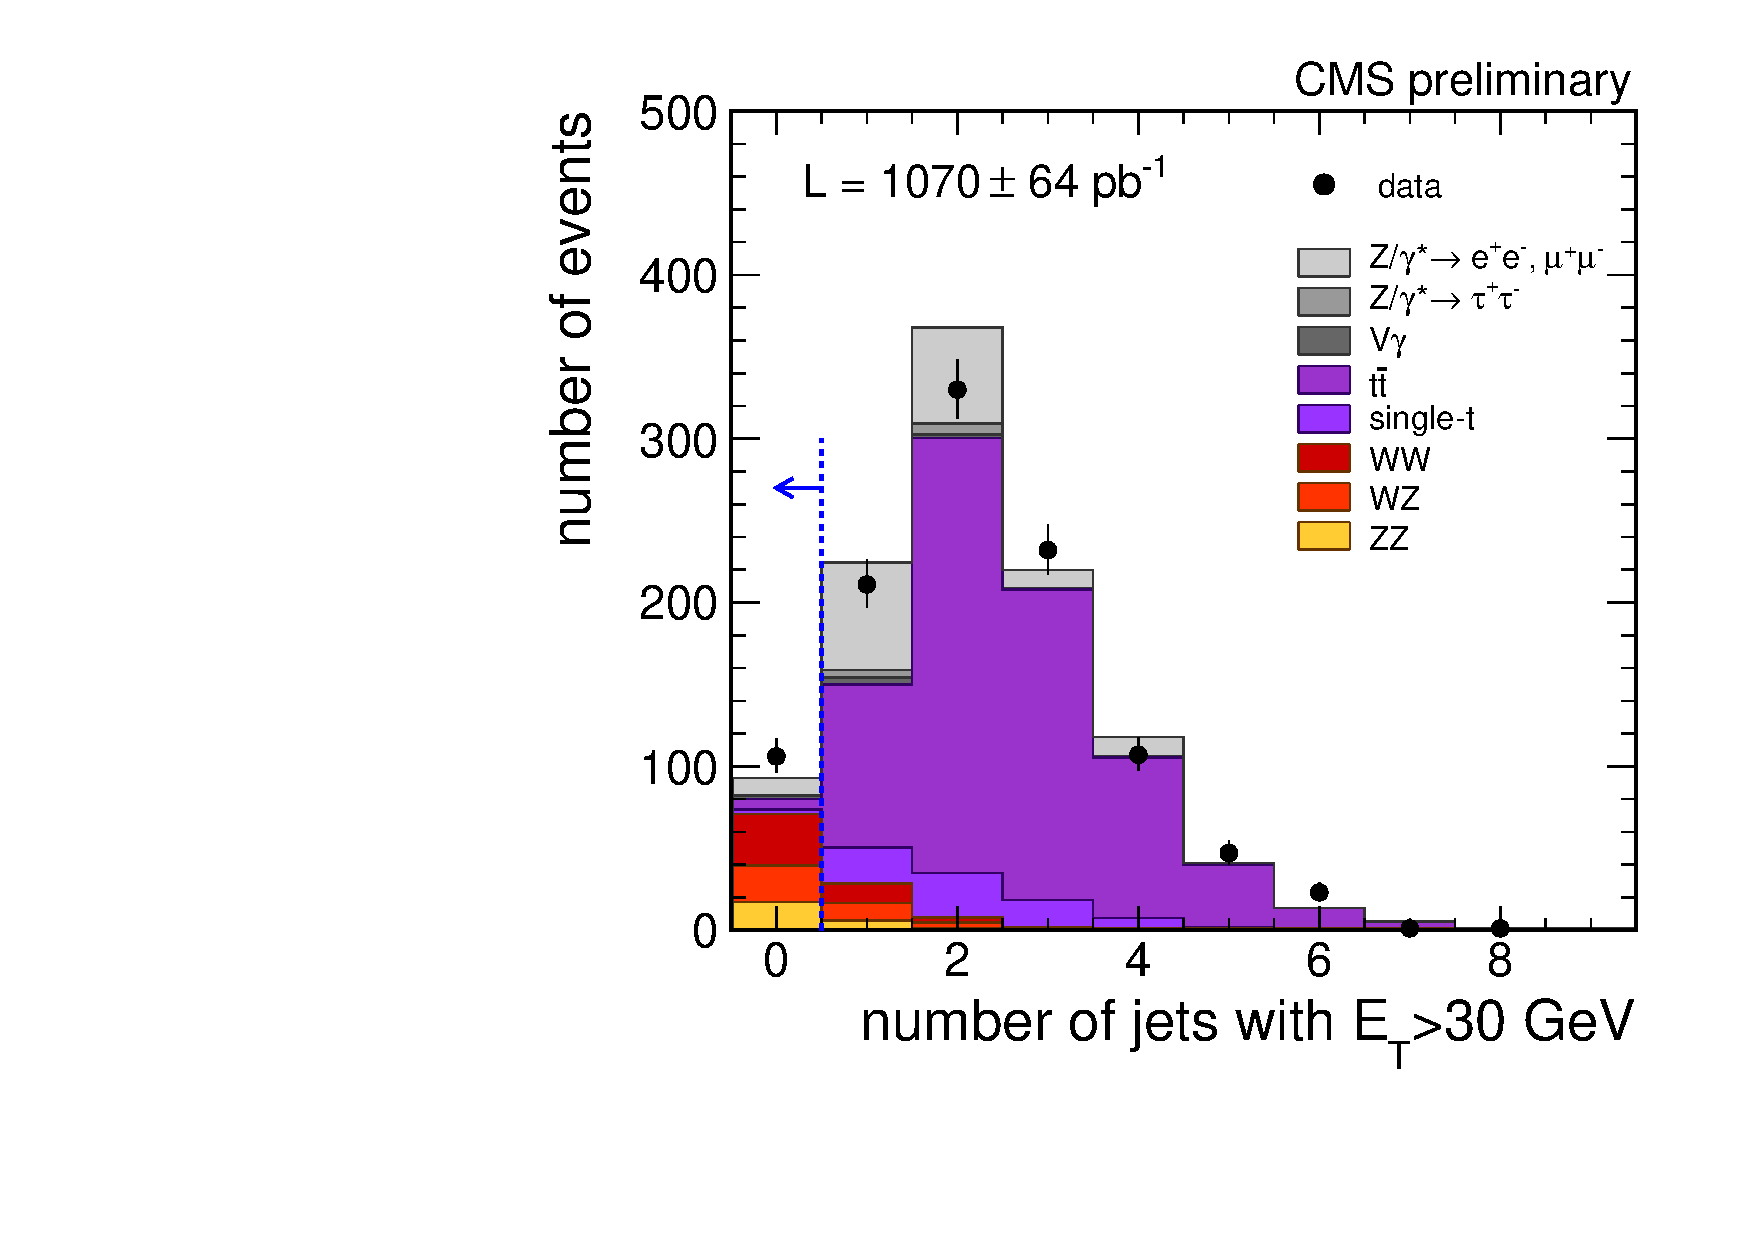
\includegraphics[width=1\linewidth]{figures/ZZ_2l2n/jMult_q30_met.pdf}
\caption{Exclusive jet multiplicity, for di-lepton events after $\QT$ and $\met$ cuts. \label{fig:ZZ_2l2n_jMult_q30_met}}
\end{minipage}
\hspace{0.5cm}
\begin{minipage}[t]{0.48\linewidth}
\centering
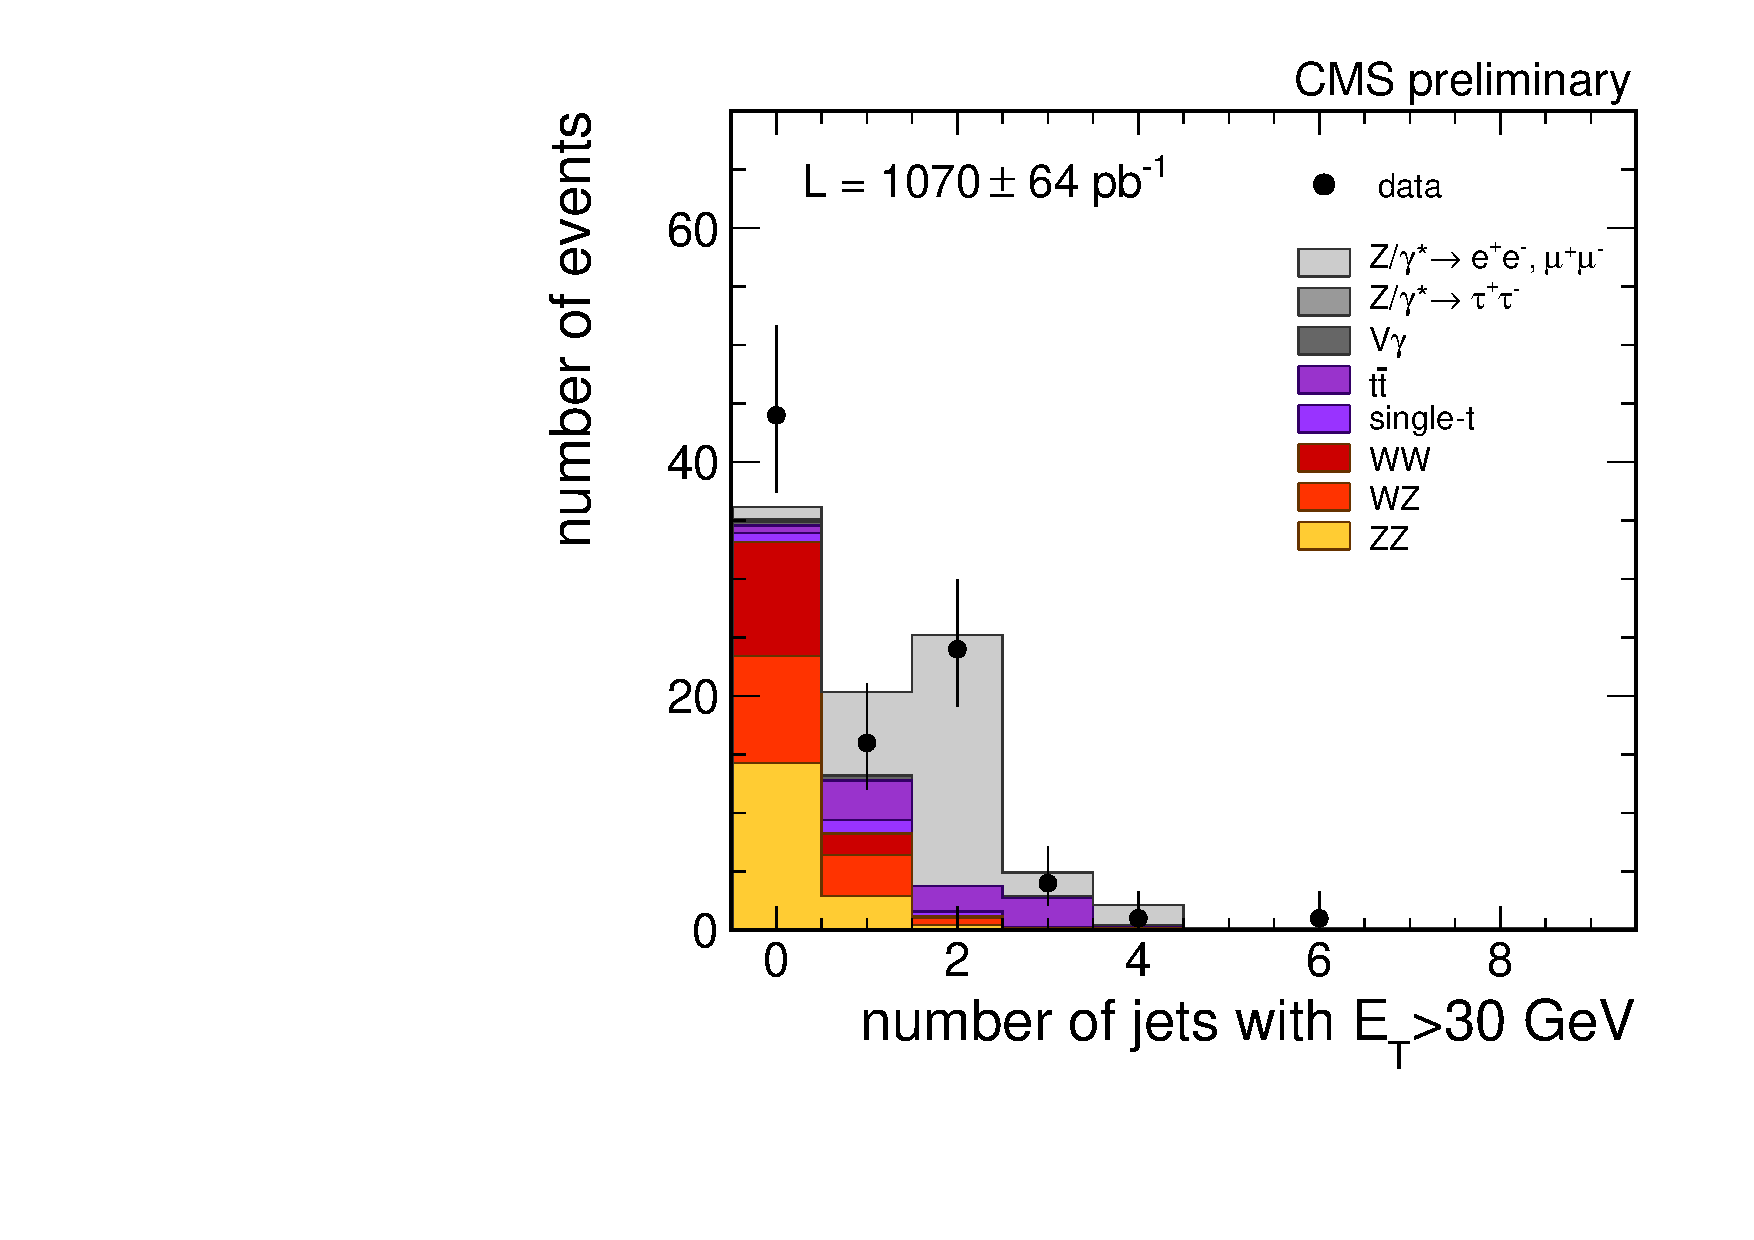
\includegraphics[width=1\linewidth]{figures/ZZ_2l2n/jMult_final.pdf}
%\hspace{.05in}
\caption{Exclusive jet multiplicity, for di-lepton events after all selections, in the $80$-$100~\GeV$ mass window. \label{fig:ZZ_2l2n_jMult_final}}
%\end{center}
\end{minipage}
\end{figure}

To fight the overwhelming $\PZ+{\mathrm {jets}}$ and Drell-Yan backgrounds we apply a jet veto and impose a strong $\met$ requirement. The jet veto energy threshold, $\ET^{\mathrm{jet}}>30~\GeV$, is chosen to stay insensitive to jets originating from pile-up events.  The $\met$ requirement, $\CORRMET>50~\GeV$, is determined to obtain, together with the jet veto, a final rejection factor of $2.5 \times 10^{5}$ against $\PZ+{\mathrm {jets}}$ and Drell-Yan backgrounds.  For convenience, we also apply a cut on the transverse momentum \QT\ of the di-lepton candidate at $30~\GeV$, which is the photon transverse energy threshold of our the $\gamma + \mathrm{jets}$ control sample; this cut has no effect once the jet veto and \CORRMET\ cuts are applied. After the jet veto and the $\QT$ cut, the $\CORRMET>50~\GeV$ cut has an efficiency of $62\%$ on the \ZZ\ signal for an additional rejection of $2\,000$ on the Drell-Yan background. The distribution of the \CORRMET\ variable after jet veto is shown on Fig.~\ref{fig:ZZ_2l2n_corrMET_jet}}, and after the $\QT$ cut on Fig.~\ref{fig:ZZ_2l2n_corrMET_q30_jet}.

The remaining $\PZ+{\mathrm {jets}}$ background is further cleaned-up by three additional kinematical cuts. To ensure the correct  balance between the $\PZ$ boson transverse momentum and the transverse missing momentum we apply a cut on the ratio of the $\MET$ to the di-lepton transverse momentum, $0.4< \MET/\QT < 1.8$, and a cut on the angle between the $\MET$ direction and the di-lepton axis, $\Delta \phi( \MET, -\VECQT )<60^{\circ}$; to reject events with a mismeasured jet we apply a cut on the angle between the $\MET$ direction and the closest jet in the event, $|\min( \Delta \phi ( \MET, { \mathrm{jet} } ) )|>20^{\circ}$. These cuts have close to 100\% efficiency on the signal. 



\begin{figure}[b]
\begin{center}
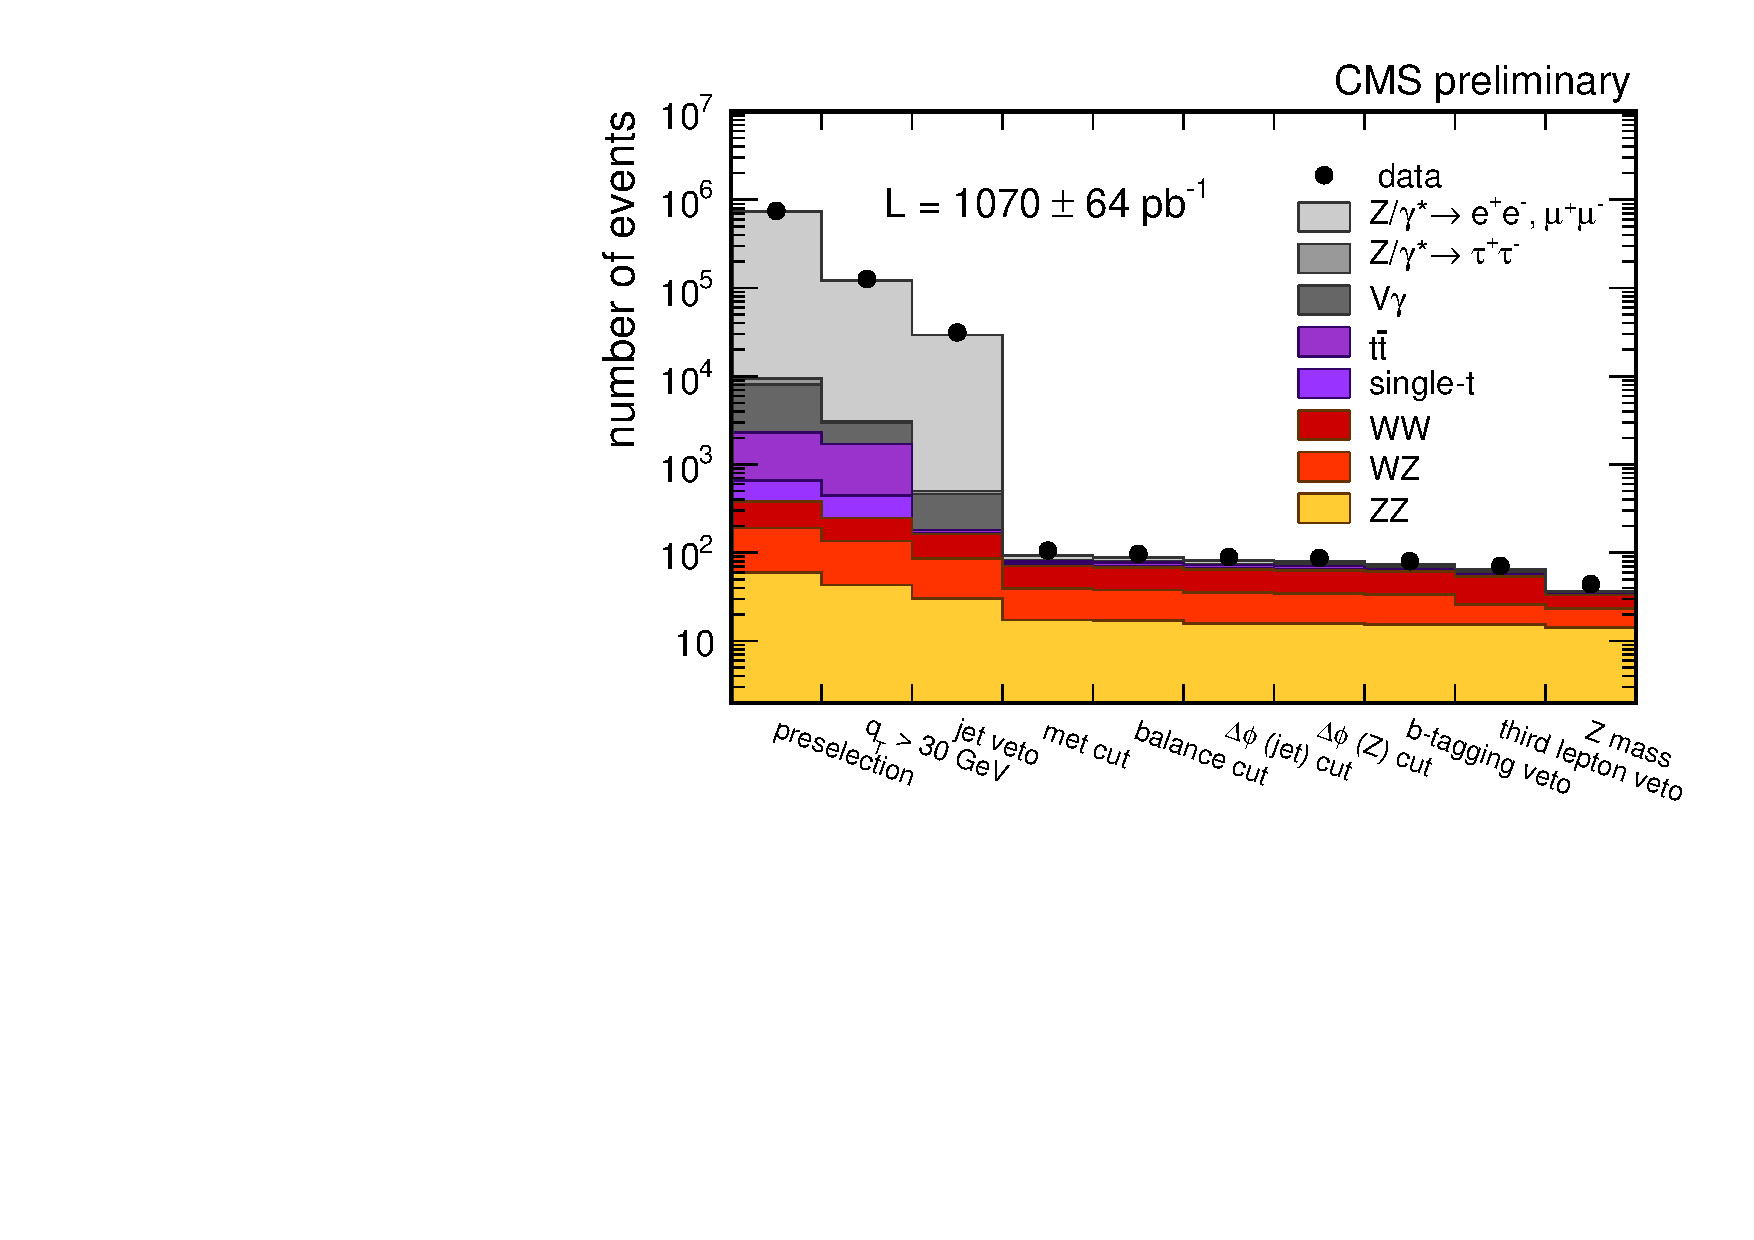
\includegraphics[width=0.70\textwidth]{figures/ZZ_2l2n/Cumul.pdf}
\hspace{.05in}
\caption{Succession of cuts in the $\ZZ\to\ell\ell\nu\nu$ analysis. \label{fig:ZZ_2l2n_cumul}}
\end{center}
\end{figure}


The top backgrounds ($t\bar{t}$ and single-top) are also strongly reduced by the jet veto.  This is illustrated by the jet-multiplicity distribution on Fig.~\ref{fig:ZZ_2l2n_jMult_q30_met}, where only the $\QT$  and the $\CORRMET$ cuts are applied. To further reduce the top backgrounds, we apply a b-tagging veto based on two b-tagging variables, one that counts the number of displaced vertices, another one based on the presence of a soft muon in a jet.  The plot on Fig.~\ref{fig:ZZ_2l2n_jMult_final} shows the jet multiplicity distribution after all kinematical cuts and b-tagging criteria applied, in the reduced $[80$-$100]~\GeV$ mass window. There is good agreement in the 2-jet and 3-jet bins, which are dominated by the $\PZ+\mathrm{jets}$ and top backgrounds, respectively. The agreement is good also in the 1-jet bin, where  $\PZ+\mathrm{jets}$ and top contribute in comparable amount to the background, which represents more than half of the sample. The 0-jet bin is dominated by diboson events, $\WW$, $\WZ$, and $\ZZ$. The $\WZ$ component is reduced by rejecting events containing at least one additional lepton with $\PT>20~\GeV$ selected with looser identification and isolation criteria.  The succession of selection cuts is illustrated on Fig.~\ref{fig:ZZ_2l2n_cumul}.

\begin{figure}[t]
\begin{minipage}[t]{0.48\linewidth}
\centering
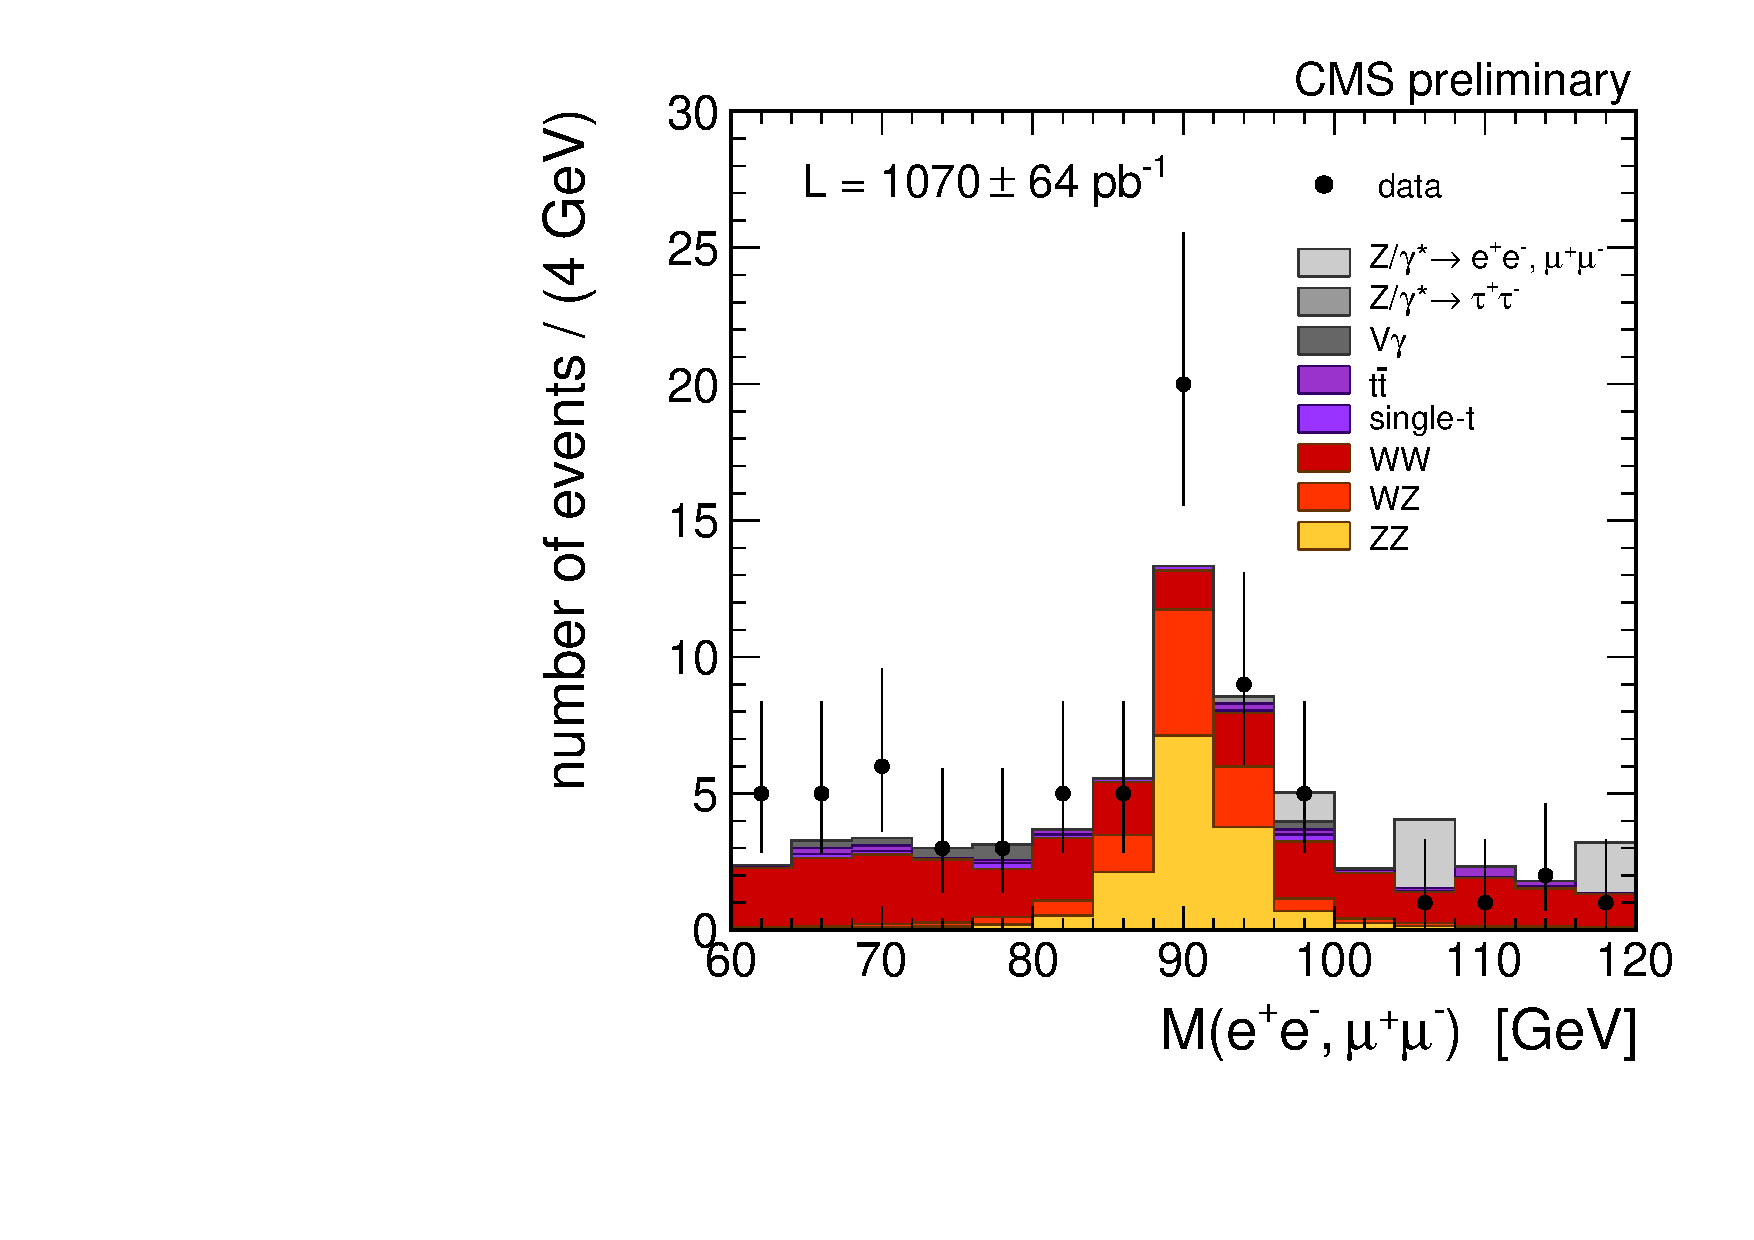
\includegraphics[width=1\linewidth]{figures/ZZ_2l2n/mll_final.pdf}
\caption{Dilepton mass spectrum for the final $\ZZ\to\ell\ell\nu\nu$ selection. \label{fig:ZZ_2l2n_mll_final}}
\end{minipage}
\hspace{0.5cm}
\begin{minipage}[t]{0.48\linewidth}
\centering
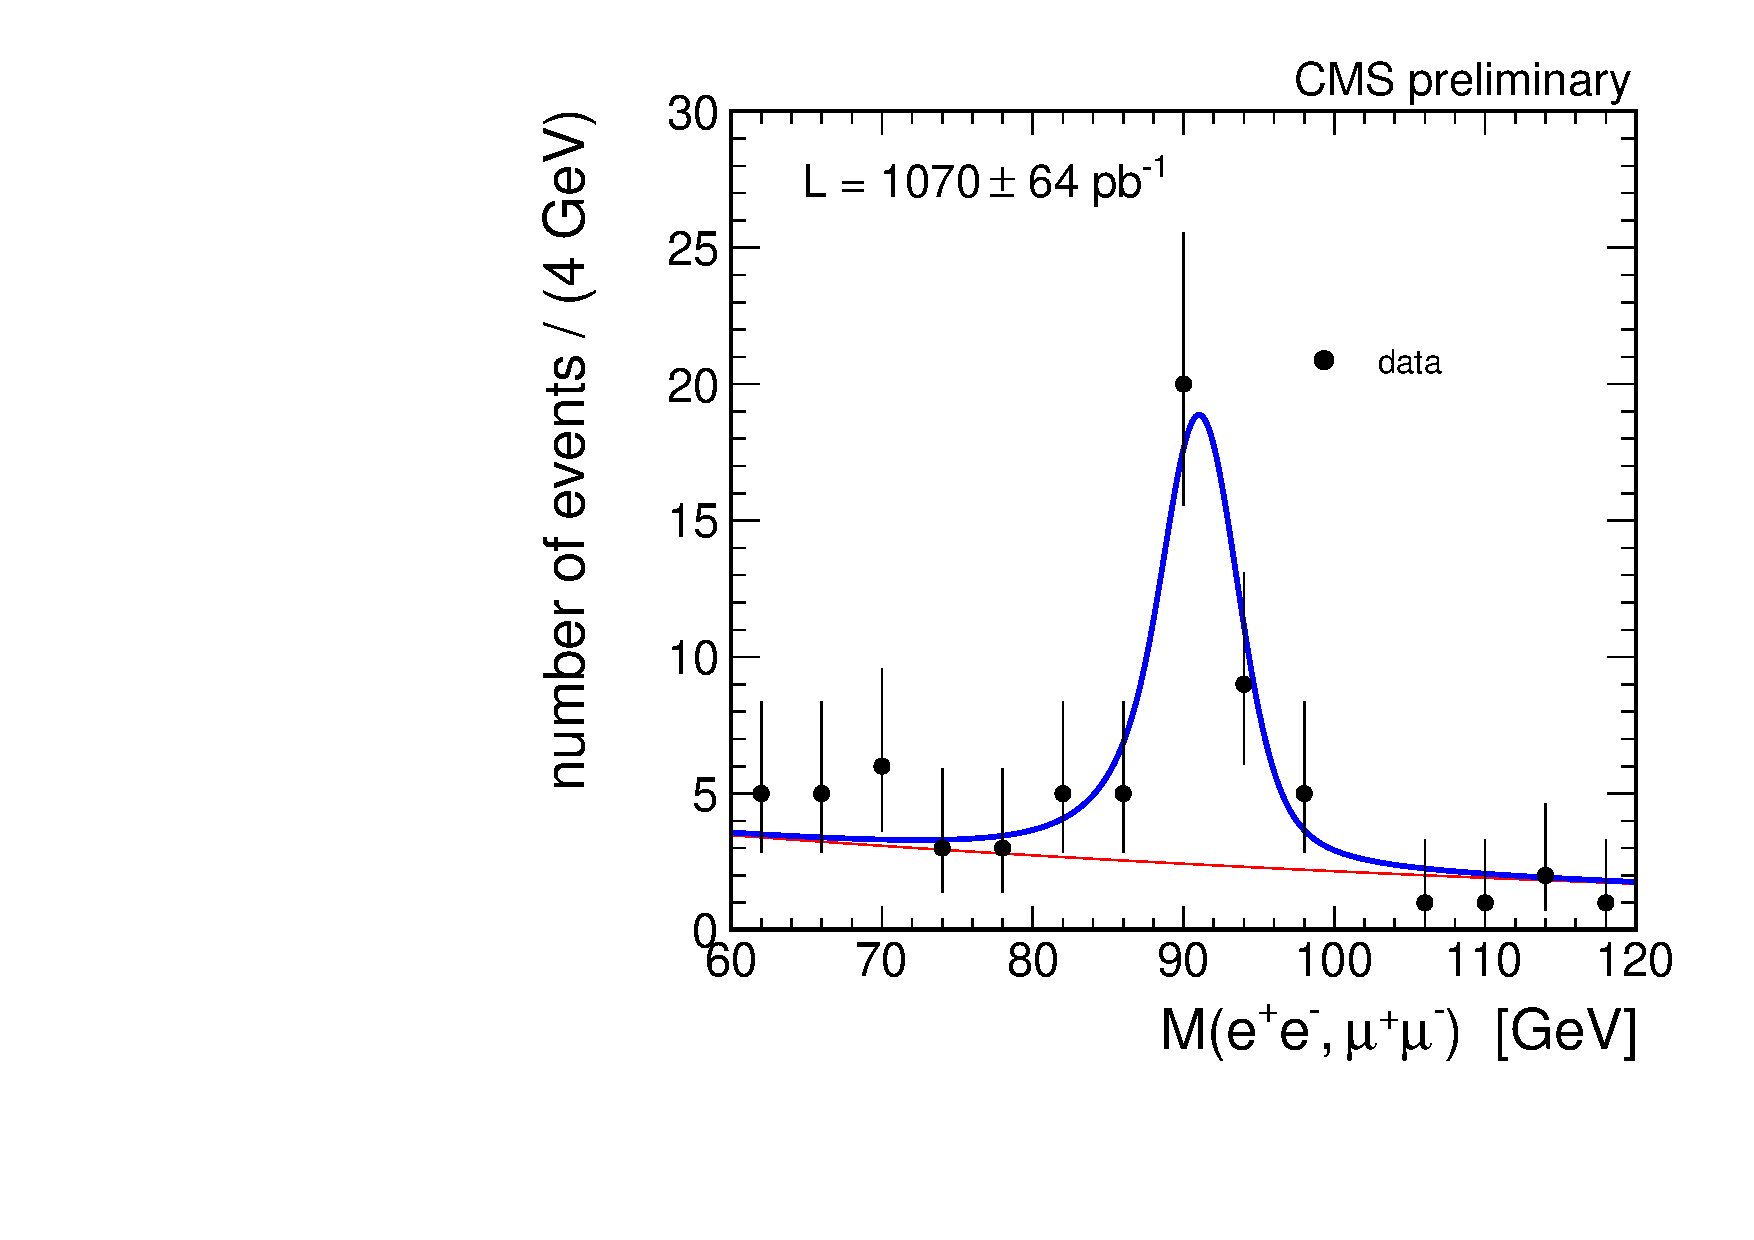
\includegraphics[width=1\linewidth]{figures/ZZ_2l2n/fitMll.pdf}
\caption{Unbinned maximum likelihood fit to the dilepton mass spectrum. \label{fig:mll_fit}}
\end{minipage}
\end{figure}

\def\NELE{\ensuremath{37}}
\def\NELEWIN{\ensuremath{23}}
\def\NMUO{\ensuremath{34}}
\def\NMUOWIN{\ensuremath{21}}

The di-lepton mass spectrum for selected events is shown on Fig.~\ref{fig:ZZ_2l2n_mll_final}.  We select \NELE\ (\NMUO) events in the electron (muon) channel, \NELEWIN\ (\NMUOWIN) of which in the reduced $[80$-$100]~\GeV$ mass window. The Monte Carlo simulation for the $\WW$, $\WZ$ and $\ZZ$ components are produced at the leading order (LO) in QCD with the Pythia event generator; a dynamical NLO/LO weight (k-factor), determined using NLO and LO differential cross-sections computed with MCFM, is applied event-by-event.  

We use an unbinned maximum likelihood fit to the di-lepton spectra to extract the peaking component and the non-peaking \WW\ background. In the fits, the \PZ\ line-shape comes from a $\PZ+\mathrm{1\,jet}$ control sample in the data, described later, and the \WW\ line-shape, from the Monte-Carlo simulation. Other non-peaking backgrounds are taken as uniform in the mass window, except for the $\PZ\to\tau^+\tau^-$ background, which found to be negligible. Because the \PZ\ line-shapes differ in the electron and muon channels due to different mass resolution functions, the fits are performed separately.  Figure~\ref{fig:mll_fit} is an illustration of a fit to the combined lepton sample using an averaged \PZ\ line-shape.   

%\begin{figure}[hbt]
%\begin{center}
%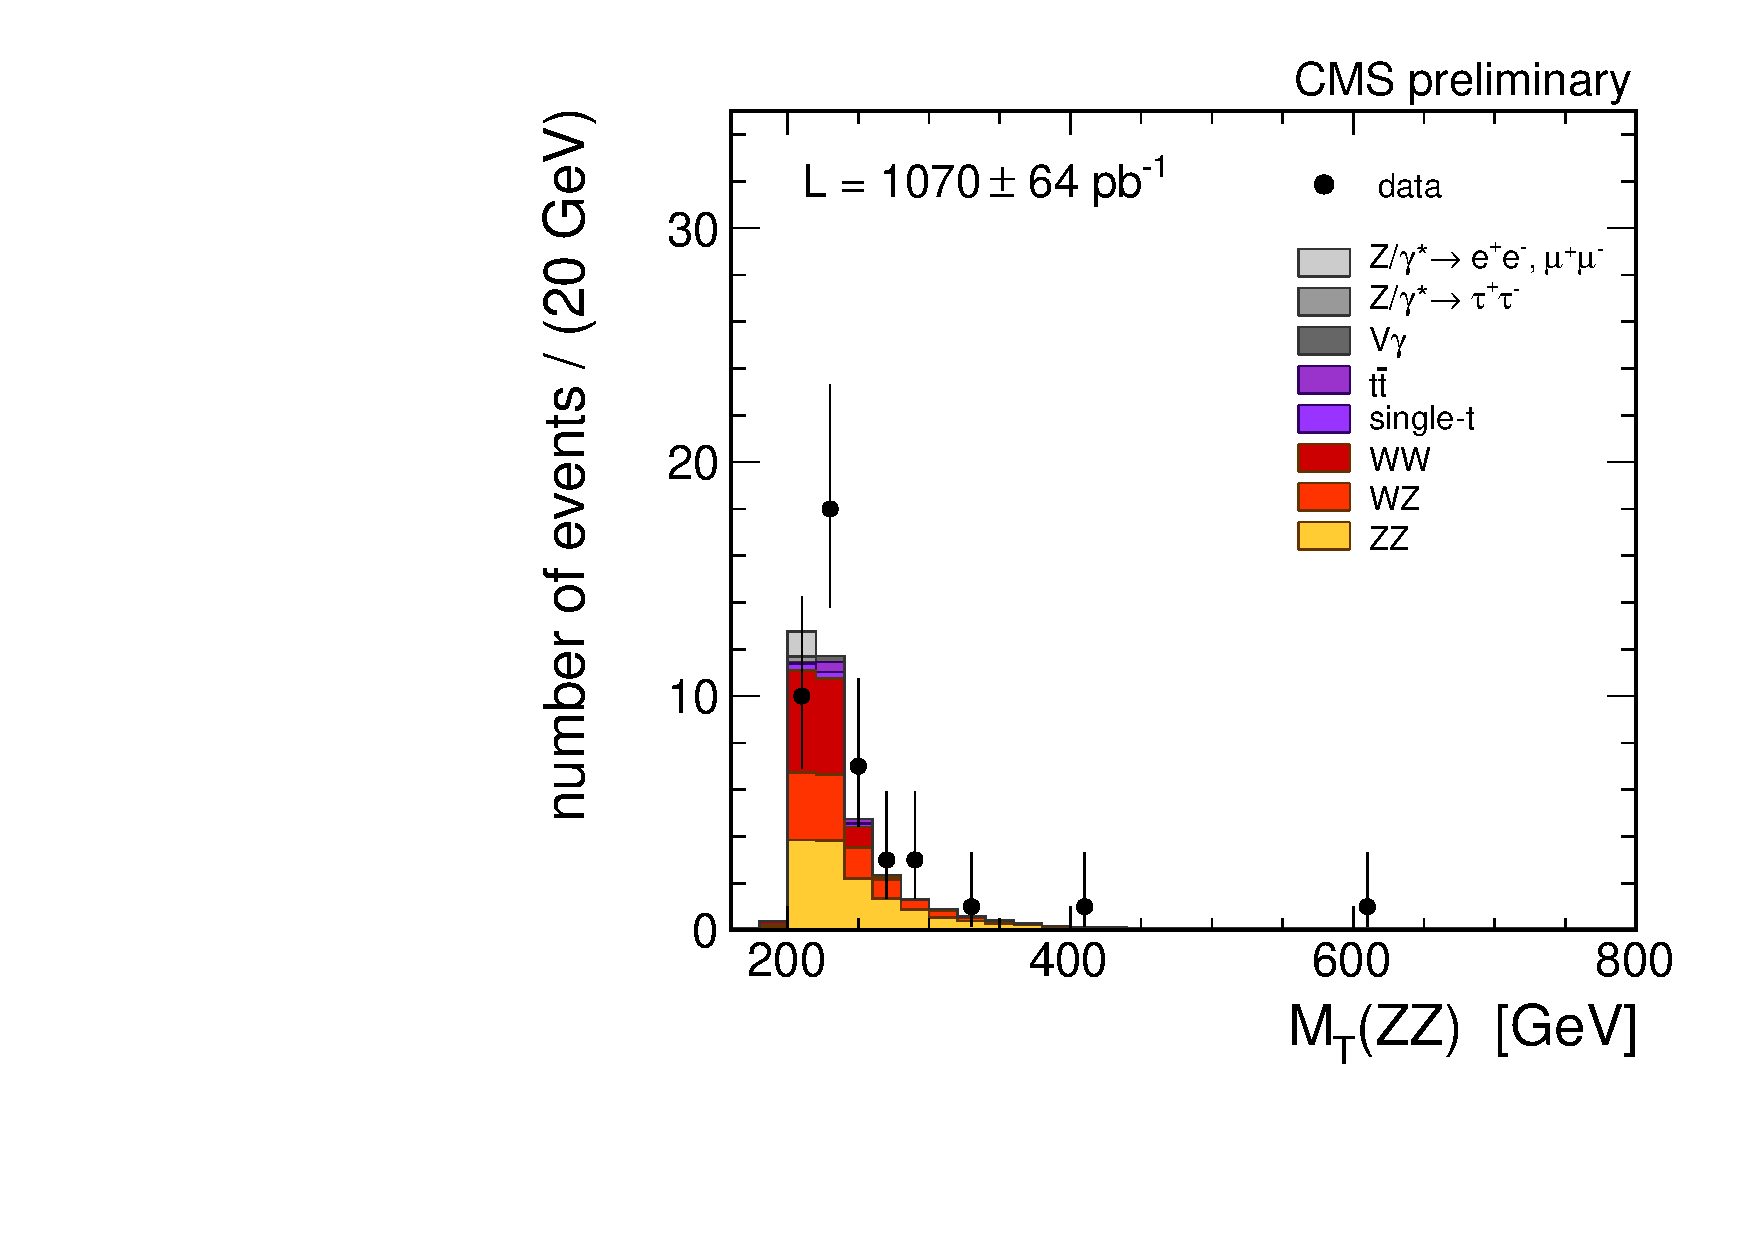
\includegraphics[width=0.70\textwidth]{figures/ZZ_2l2n/mTZZ_final.pdf}
%\hspace{.05in}
%\caption{$ZZ$ transverse  mass for the final $\ZZ\to\ell\ell\nu\nu$ selection in the $[\,80\,$-$\,100\,]~\GeV$ mass window. \label{fig:ZZ_2l2n_mTZZ_final}}
%\end{center}
%\end{figure}

%The $(\PZ,\met)$ transverse mass distribution for the 14 events in a restricted $[\,80\,$-$\,100\,]~\GeV$ di-lepton mass window around the $Z$ peak (9 and 5 in the electron and muon channels, respectively) is shown in Fig.~\ref{fig:ZZ_2l2n_mTZZ_final}.  The level of Drell Yan, $\PZ+{\mathrm{jets}}$, $Z\to\tau\tau$ and $\PW+{\mathrm{jets}}$ backgrounds is expected to be negligible from the simulation.  The background of $t\bar{t}$ events is estimated at $0.5\pm0.3$ where the error comes from the Monte Carlo statistics. The expected number of diboson events in the restricted mass window is 3.2, 4.1 and 6.5 for the $\WW$, $\WZ$ and $\ZZ$ modes, respectively.  

\subsection{Backgrounds}

Most considered backgrounds are estimated or cross-checked using data-driven methods. 

The $\PW+\mathrm{jets}$ background is estimated using a method where the electron fake rate is measured from loose electron candidates in a pure QCD background sample, and applied to a sample of $\PZ$ candidates with one loose electron candidate. The $\PW\gamma$ background is estimated from simulation. We check that adding photon conversion rejection requirements to the electron identification criteria has no impact on the selected sample. These backgrounds are found to contribute only to the non-peaking background in the electron channel: $3.5\pm1.6$ and $1.5\pm0.5$ events for $\PW+\mathrm{jets}$ and $\PW+\gamma$, respectively. 

The $\PZ\gamma\to\ell^+\ell^-\gamma$ background, where one of the leptons falls outside acceptance, is negligible in the muon channel and very small in the electron channel. Events with both leptons in acceptance and surviving all the cuts, contribute to the peaking background. This contribution is estimated from the Monte-Carlo simulation: $0.3\pm0.2$  ($0.1\pm0.1$) events in the electron (muon) channels, with large errors.  

The top background is estimated from the centrally measured b-tagging efficiency and the fraction of events rejected by our b-tagging requirements in a top-enriched control sample obtained by inverting the di-lepton mass window and requiring at least two hard jets in the event. The top contribution to the non-peaking background amounts to $0.7\pm0.4$ and $1.0\pm0.5$ events in the electron and muon channels, respectively. 

The Drell-Yan background is estimated by extrapolating the \CORRMET\ distribution from the Drell-Yan dominated region to the signal region. The functional form of the \CORRMET\ distribution for the Drell-Yan is exercised on the Monte-Carlo simulation (we adopt a three-parameter Novosibirsk function), fitted on the data below $30~\GeV$ and integrated above the cut value of $50~\GeV$. We obtain $3.6\pm0.9$  and $1.6\pm0.4$ events in the electron and muon channels, respectively. We cross-check the contribution of Drell-Yan and $\PZ + {\mathrm {jets}}$ backgrounds using a sample of QCD events in the data containing one hard isolated photon with $\ET^{\gamma}>30~\GeV$.  Photons are selected with very tight identification and isolation criteria to get a reasonable photon purity. We apply the jet veto and we re-weight the events in the control sample so that the photon transverse momentum spectrum matches that of the $\PZ$ boson. We then normalize the $\CORRMET$ distribution of the $\gamma+\mathrm{jets}$ sample to that of the $\PZ + {\mathrm {jets}}$ in a region around the maximum of the distribution. The contribution of $\PZ\gamma \to \nu\nu\gamma$ events, which dominates the tails of the $\CORRMET$ distribution in the control sample, is estimated from the Monte-Carlo simulation normalized to the CMS measurement of the $\PZ\gamma$ production cross-section, and subtracted. The experimental error of $40\%$ on the $\PZ\gamma$ cross-section is propagated to the final background estimates. 
We obtain background estimates that are consistent, within errors. The $\gamma+\mathrm{jets}$ control sample ensures that there is no unexpected source of tails in the \CORRMET\ distribution. 

The background-subtracted \WZ/\ZZ\ yields are $${N^{\WZ/\ZZ}}_{\Pe}=\NElePeakingWithWZ\ \ \mathrm{and}\ \ {N^{\WZ/\ZZ}}_{\Pgm}=\NMuoPeakingWithWZ,$$
and the background-subtracted \WW\ yields are $${N^{\WW}}_{\Pe} = \NEleNonPeaking\ \ \mathrm{and}\ \ {N^{\WW}}_{\Pgm}=\NMuoNonPeaking,$$ in the electron and muon channels, respectively.

%We can then compare, on both samples, the effect of the $\CORRMET$ and other kinematical cuts.  

\subsection{Efficiencies}

The values of di-lepton selection efficiency ${(\mathcal{A}\times\varepsilon)^{\ZZ\,(\WZ)}}_{\ell\ell}$, determined from the simulated \ZZ\ (\WZ) samples with dynamical NLO/LO re-weighting, are  $39.6\%$ ($36.7\%$) and $58.2\%$ ($53.3\%$) in the electron and muon channels, respectively. The values of ${(\mathcal{A}\times\varepsilon)^{\ZZ\,(\WZ)}}_{\ell,\mathrm{sim}}$ after all selections are obtained from the simulation with a dynamical NLO/LO re-weighting that takes into account the effect of the jet veto on the NLO cross-sections. We find $8.5\%$ ($2.0\%$) and $11.0\%$ ($2.8\%$) for the \ZZ\ (\WZ) mode in the electron and muon channels, respectively. 

We use ratios of efficiencies on control samples in the data and the simulation, $\rho = \epsilon_{\mathrm{data}}/\epsilon_{\mathrm{sim}}$, as signal efficiciency correction factors, $\varepsilon = \rho \times \varepsilon_{\mathrm{sim}}$. 

The correction factors for lepton trigger, reconstruction, identification and isolation are determined by the tag-and-probe method. The largest correction is in the electron channel, $\rho=0.931\pm0.002$.  The di-lepton trigger efficiencies are estimated assuming that the lepton trigger efficiencies factorize: $98.8\pm0.3\%$ and $92.2\pm0.1\%$ for di-electron and di-muon triggers, respectively.  The tag-and-probe results are also exploited to correct the third-lepton veto efficiency on the \WZ\ sample, $\rho=1.015\pm0.009$. 

We use the ratio of jet-veto efficiencies on $\PZ+\mathrm{jets}$ samples in the data and the NLO simulation to correct the jet veto efficiency on the \ZZ\ and \WZ\ simulated samples. We check the validity of the method by applying it to a $\PZ+\mathrm{jets}$ sample generated at the LO with Pythia, and by varying the jet-veto threshold. The same control sample with a $\met$ cut is exploited to determine the b-tagging veto efficiency on non-top events, $\sim95\%$ with a correction factor consistent with one. The third-lepton veto efficiency on \ZZ\ events, close to 100\%, does not need correction.  

For the study of the \CORRMET\ and the three kinematical cuts, we construct a control sample from the sample of \PZ\ events with $\QT>30~\GeV$ and exactly one jet of transverse energy larger than $30~\GeV$. 
%As described above, this jet is attributed to the hard-scatter vertex; therefore, its contribution is not scaled down in the computation of the \PUMET\ variable.  
We ignore the jet in the computation of the \PUMET\ variable and in the jet veto as if the jet went undetected, and we re-weight events to match the \PZ\ transverse momentum spectrum of the \ZZ\ signal.  
%We do so in the data and in the Monte-Carlo simulation and we use 
Data/simulation efficiency ratios are then obtained for the \CORRMET\ and kinematical cuts, 
applied one after the other. 
The largest discrepancy ($\rho\sim0.75$) is found for the \CORRMET\ cut. This results from the imperfect modeling of the off-time pile-up in the simulation; the scaling involved in the computation of the \CORRMET\ variable has an impact on events with genuine missing transverse energy that is larger in the data than in the simulation. We check this assumption by performing the analysis with the un-scaled \PUMETMIN\ variable instead of \CORRMET. To obtain the same rejection factor on the Drell-Yan background,  the cut on \PUMETMIN\ must be placed $15~\GeV$ higher in the data, which leads indeed to a consistent relative loss of signal efficiency.   The di-lepton spectra obtained at the end of the selection on these control samples in the data provide the \PZ\ line-shapes for the unbinned maximum likelihood fits.   

The overall efficiency correction factors are, for the \ZZ\ mode, 
$${\rho^{\ZZ}}_{\Pe}=\RhoEleZZ\ \ \mathrm{and}\ \ {\rho^{\ZZ}}_{\Pgm}=\RhoMuoZZ,$$
and, for the \WZ\ mode,
$${\rho^{\WZ}}_{\Pe}=\RhoEleWZ\ \ \mathrm{and}\ \ {\rho^{\WZ}}_{\Pgm}=\RhoMuoWZ,$$
in the electron and muon channels, respectively.

The numbers of \WZ\ events are estimated using the CMS results on \WZ\ in the $3\ell\nu$ channel described in Ref.~\cite{CMS-PAS-EWK-11-010} and the ${(\mathcal{A} \times \varepsilon)^{\WZ}}_{\ell,\mathrm{sim}} \times {\rho^{\WZ}}_{\ell}$ products. We find $ {N^{\WZ}}_{\Pe} = \NbkgZWInZZee $ and $ {N^{\WZ}}_{\Pgm} =  \NbkgZWInZZmm$ in the electron and muon channels, respectively. We obtain consistent but less precise results from the numbers of events rejected by the third lepton veto.

%All other selection cuts have no impact on the signal efficiency, and therefore lead to negligible systematic uncertainties. 

\subsection{Production Cross-Sections}

The production cross-section times branching ratio measurements are based on the equation 
$$
   \SIGBRZZll = \frac{{N^{\WZ/\ZZ}}_{\ell} - {N^{\WZ}}_{\ell} }{ {(\mathcal{A} \times \varepsilon)^{\ZZ}}_{\ell,\mathrm{sim}} \times {\rho^{\ZZ}}_{\ell} \times \mathcal{L} }\ \, , 
$$
with $\ell=\Pe$ or $\ell = \Pgm$. We measure
\begin{eqnarray}
  \SIGBRZZee &=& \ZZElecXsect , \nonumber \\
  \SIGBRZZmm &=& \ZZMuonXsect , \nonumber 
\end{eqnarray}
and, for the combined lepton channel, 
\begin{eqnarray}
  \SIGBRZZll &=& \ZZCombXsect  , \nonumber
\end{eqnarray}
with $\ell$ denotes either electron or muon. 

Using the known branching fractions of the \PZ\ boson we obtain a measurement of the $\pp \to \ZZ $ inclusive production cross-section, 
\begin{eqnarray}
  \SIGZZ &=& \ZZXsect \, .\nonumber
\end{eqnarray}

This result is in agreement with the Standard Model expectation, $\sigma( \pp \to \ZZ ) = 5.9~\mathrm{pb}^{-1}$, computed at the next-to-leading order in perturbative QCD with the MCFM program.

\subsection{Systematic Uncertainties}

\def\GlobSystElec{ \ensuremath{ 18.9\%  }\xspace}
\def\GlobSystMuon{ \ensuremath{ 16.2\%  }\xspace}
\def\GlobSystComb{ \ensuremath{ 17.6\%  }\xspace}

We hereby mention only the main source of systematic uncertainties.

The uncertainties on di-lepton acceptance due to parton density functions are estimated at the 90\% confidence level with the latest MSTW-LO PDF set and lead to a relative uncertainty of $1.5\%$ on the cross-section measurements.  The electron and muon energy/momentum scales induce relative selection uncertainties of $2(3)\%$ for electrons in the EB (EE) and $3\%$ for muons, which propagate to a relative uncertainty of $1.5\%$ on the cross-section measurements.  Uncertainties on lepton reconstruction, identification and isolation efficiency correction factors from the tag-and-probe are propagated to the cross-section measurements. 

The jet veto efficiency depends on the jet energy scale, which is known to $3\%$ at the veto threshold $\ET=30~\GeV$. This translates to a $3.4\%$ uncertainty on the jet veto efficiency, which in turn propagates as a \JVUncEffect relative uncertainty on the cross-section measurements. An additionnal uncertainty of $0.6\%$ is assigned to the jet veto efficiency correction factor obtained from the $\PZ+\mathrm{jets}$ control sample.

The missing transverse energy requirement is an important source of systematic uncertainty on the signal selection efficiency.  We do not correct for the difference in efficiency of the \CORRMET\ cut on the \ZZ\ signal and the $\PZ+1$-jet control sample in the simulation, which is 8.8\%, because part or all of the difference may be of physical origin, but we take it as a systematic uncertainty.  We also take the variation of signal efficiency between two samples reconstructed with a difference of two pile-up vertices around the average as a systematic uncertainty. The total systematic uncertainty due to the \MET\ requirement is 11.9\%. 

The peaking backgrounds are major sources of uncertainty on the cross-section measurements.   The relative uncertainties on the Drell-Yan background are $28\%$ and $25\%$ for the electron and muon channels, respectively, translating into about $6\%$ on the cross-section measurements. The relative uncertainties on the \WZ\ measurements propagated to the cross-sections amount to $4.4\%$ and $5.8\%$, respectively. The total uncertainties due to peaking backgrounds are $14.3\%$ and $10.6\%$, respectively. The uncertainties on non-peaking backgrounds have little impact on the final cross-section results. 

The systematics uncertainties are added in quadrature to give an overall uncertainty of \GlobSystElec\ for the electron channel, \GlobSystMuon\ for the muon channel and \GlobSystComb\ for the combined lepton channel.

The relative uncertainty on the luminosity is estimated to 6\% for the present 2011 data set.

\subsection{Limits on Anomalous Triple-Gauge Couplings}

The \ZZ\ production process provides a way to probe the neutral trilinear gauge couplings at the ZZZ and $\ZZ\gamma$ vertices, which are forbidden at the tree level in the Standard Model.

The neutral trilinear gauge couplings are modelized in an effective Lagrangian by operators, each associated to an anomalous coupling constant.  It is usual to consider two coupling constants for each $\PZ\PZ\PV$ vertex,  $f_{4}^{\PV}$ and $f_{5}^{\PV}$ where $\PV = \PZ,\, \gamma$, associated to operators that are invariant or not under CP symmetry, respectively.  The presence of anomalous couplings modifies the boson spectrum at large transverse momenta, as illustrated on Fig.~\ref{fig:ZZZaTGC_ZPt}, and results in general in an enhancement of the total diboson production cross-section.  We hereby establish limits on a possible enhancement of the total production cross-section given the observations, and translate these limits into contours in the space of the $f_{4}^{\PZ}$ and $f_{5}^{\PZ}$ anomalous coupling constants.

Limits on a possible enhancement of the total cross-section are computed using an hybrid frequentist/Bayesian approach. The null hypothesis $H_0$  corresponds to the Standard Model prediction; the alternate hypothesis $H_1$, to an anomal \ZZ\ production cross-section. Let $r$ be the ratio of the enhanced to the SM-expected cross-sections.  We construct a test-statistics $\mbox{LLR}=-\ln{Q}$, where $Q$ is the likelihood ratio for null over alternate hypotheses. The likelihood functions are Poisson probabilities of observing the actual number of events under the given hypothesis. Sources of systematic uncertainties are considered as nuisance parameters that are integrated out assuming log-normal priors. 

Large numbers of pseudo-experiments are generated to determine the distributions of the test statistics $\mbox{LLR}$ for given values of $r$.  The consistency with the Standard Model is measured as the probability $P_0$ to obtain $\mbox{LLR}>0$ for $r=1$. The inconsistency with the Standard Model for a given value of $r>1$ is measured as the probability $P_1(r)$ to obtain $\mbox{LLR}<0$. Let $\alpha$ be the considered confidence level.  The limit with confidence level $\alpha$ is defined as the smallest value of $r$ for which the ratio $P_1/P_0$ equals $1-\alpha$.  

We obtain limits of $2.3$ and $1.6$ on the $r$ parameter at the  $95\%$ and $68\%$ confidence level, respectively. These values are used to set limits on anomalous triple gauge parameters $f_{4}^{\PZ}$ and $f_{5}^{\PZ}$. For each point in the ($f_{4}^{\PZ},f_{5}^{\PZ}$) plane we determine the value of $r$ by re-weighting the selected \ZZ\ events from the simulation according to the invariant mass of the \ZZ\ system. Weights are computed using the Baur generator with no energy-dependent form factor.  The regions consistent with our limits on $r$ are delimited by the approximate ellipses shown on Fig.~\ref{fig:ZZZaTGC_2D}. The regions inside the ellipses are consistent with the observations with the quoted confidence.  Unidimensional limits on   $f_{4}^{\PZ}$ and $f_{5}^{\PZ}$ are: 
\begin{table}[h]
  \begin{center}
    \begin{tabular} { |c|c|c| }
      \hline
      confidence level & $f_{4}^{\PZ}$ limits & $f_{5}^{\PZ}$ limits \\
      \hline\hline
      $95 \%$ C.L. & \FqLimTwoSig & \FcLimTwoSig \\
      $68 \%$ C.L. & \FqLimOneSig & \FcLimOneSig \\
      \hline
    \end{tabular}
  \end{center}
\end{table}

\begin{figure}[h]
\begin{minipage}[t]{0.48\linewidth}
\centering
    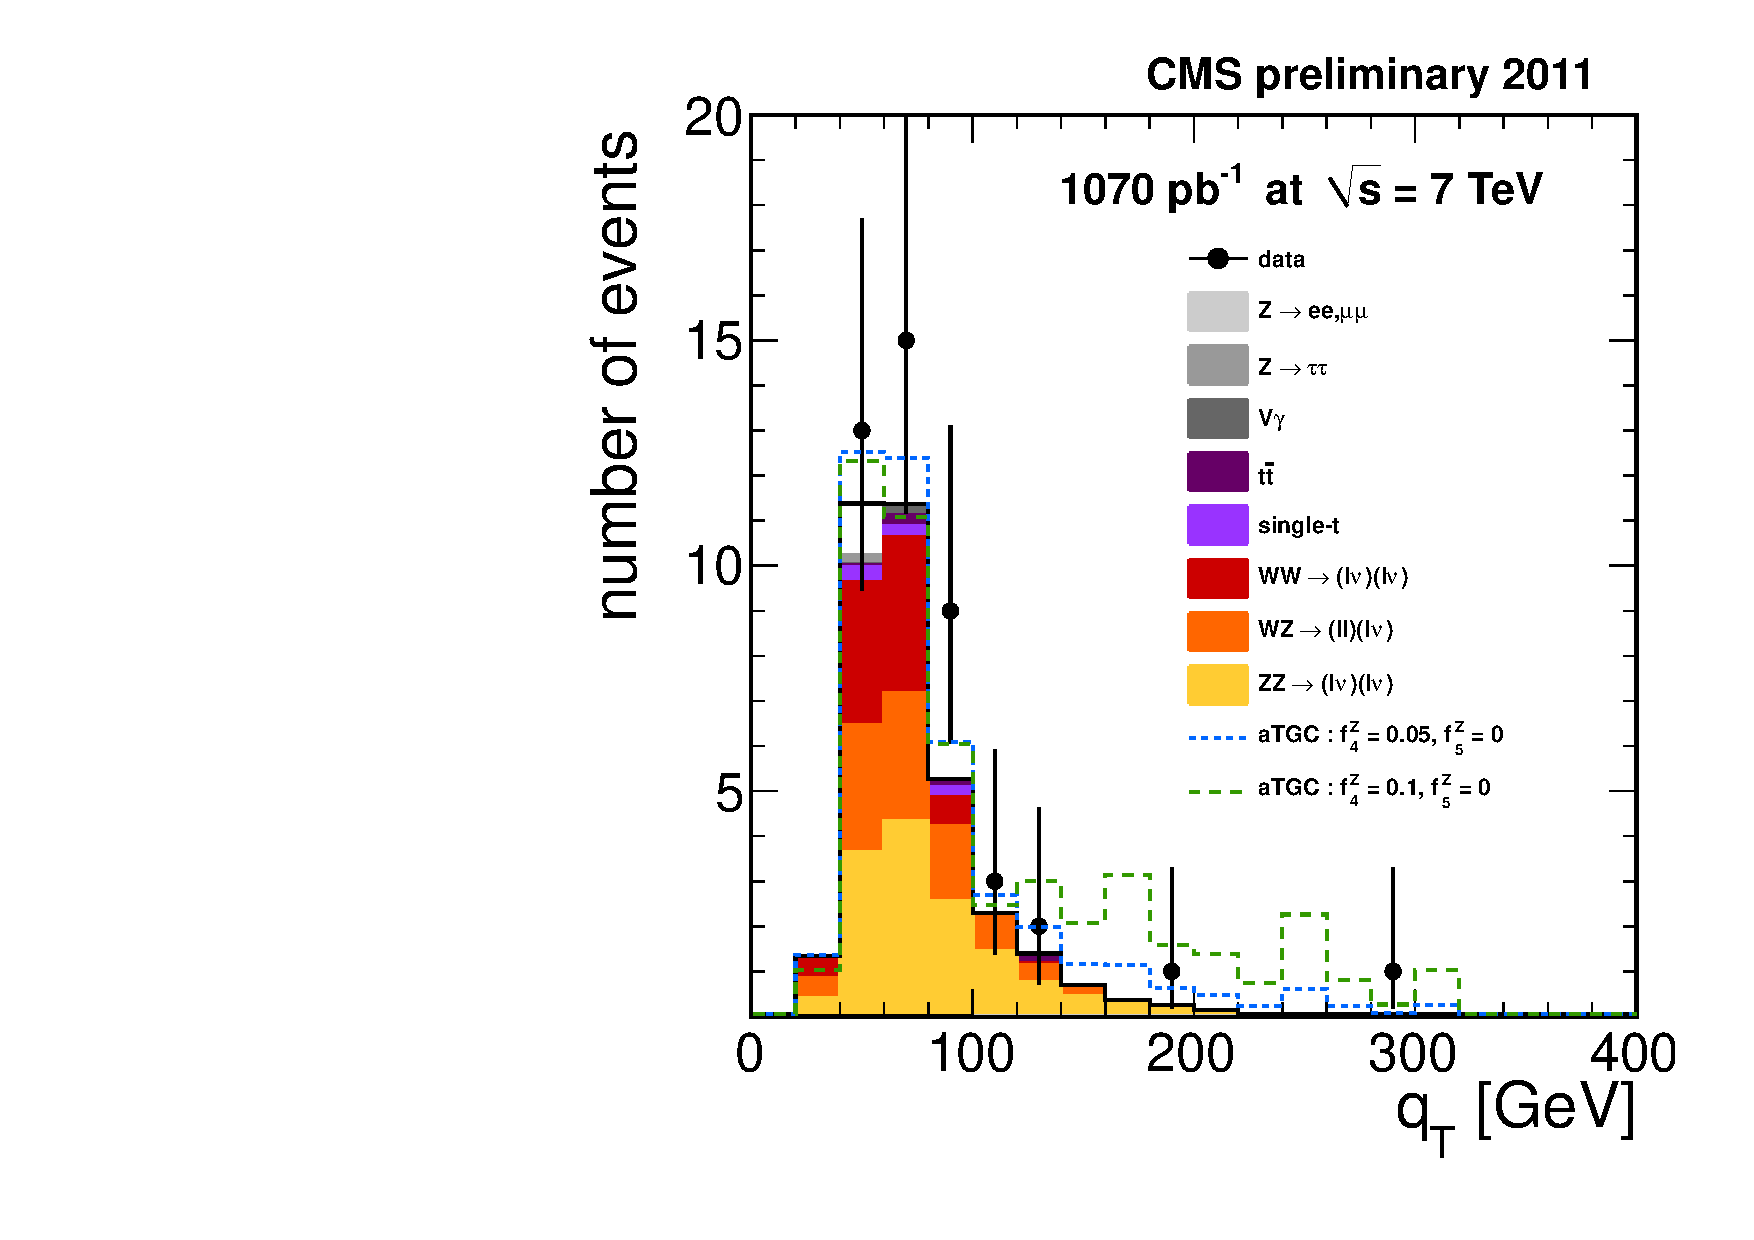
\includegraphics[width=1\textwidth]{figures/ZZ_2l2n/ZPtWithATGCs.pdf}
    \caption{ Transverse momentum of the \PZ\ boson after all selections, with examples of predictions with anomalous couplings. 
      \label{fig:ZZZaTGC_ZPt}}
\end{minipage}
\hspace{0.5cm}
\begin{minipage}[t]{0.48\linewidth}
\centering
    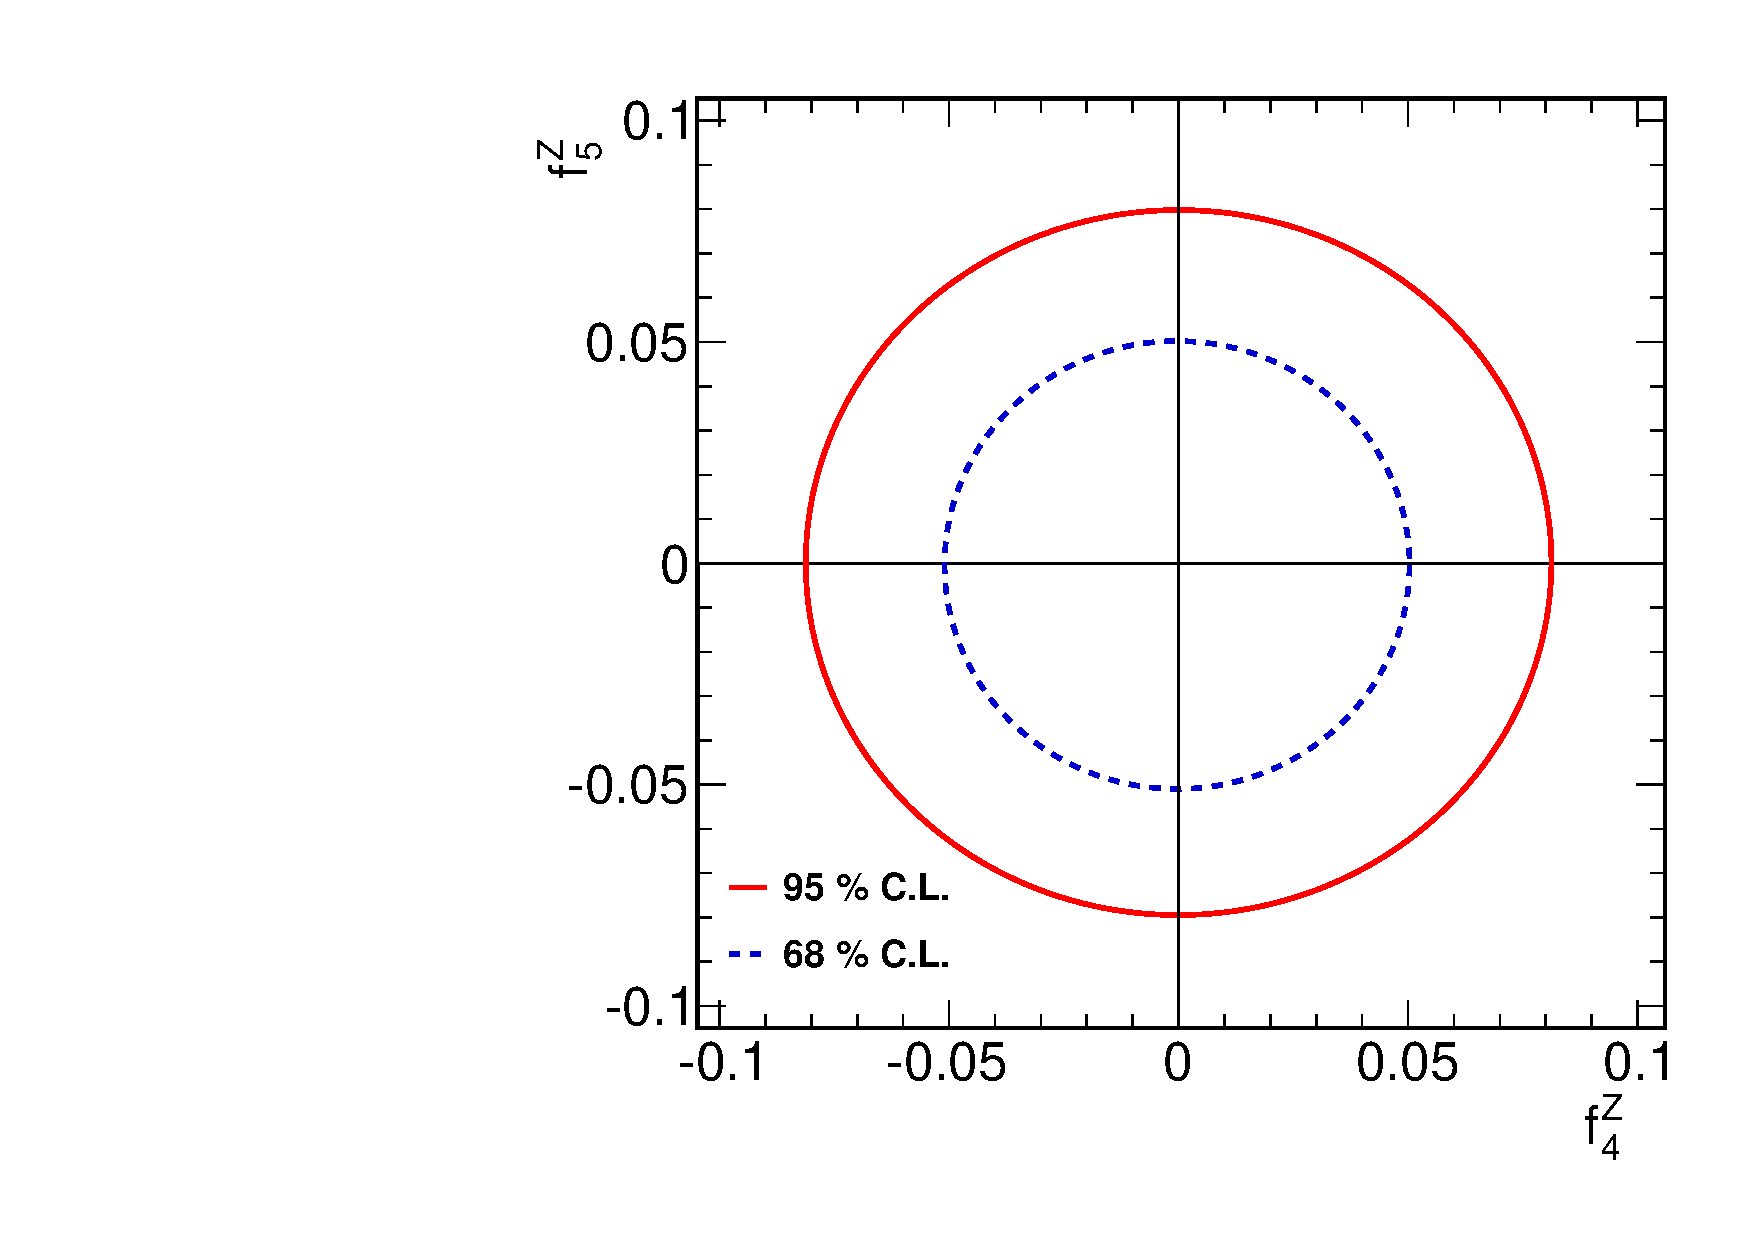
\includegraphics[width=0.95\textwidth]{figures/ZZ_2l2n/ZZZaTGC.pdf}
    \caption{ Two-dimensional limits on the $f_{4}^{\PZ}$ and $f_{5}^{\PZ}$ anomalous couplings.
      \label{fig:ZZZaTGC_2D}}
\end{minipage}
\end{figure}
